\documentclass[10pt,twocolumn,letterpaper]{article}
\usepackage{hktem}

\title{보고서 제목}
\author{정상혁\\고려대학교 지리교육과\\\email{nacl31566@korea.ac.kr}}

\begin{document}
\maketitle

\begin{abstract}
이 템플릿은 CVPR 형식을 참고해 과제물과 짧은 보고서 작성에 맞게 단순화한 한국어 \LaTeX{} 템플릿입니다. XeLaTeX 또는 LuaLaTeX으로 컴파일하며, 본문 기본 글꼴은 나눔명조로 설정되어 있습니다.
\end{abstract}

\section{Code Description}

순전파(forward pass)에서는 은닉 표현 \(h\)가 아핀 변환 \(XW_1 + b_1\)에 ReLU 활성화 함수를 적용하여 계산된다. 이렇게 얻어진 은닉 표현은 다시 또 하나의 아핀 연산 \(hW_2 + b_2\)을 통해 변환되어 소프트맥스 분류를 위한 클래스 점수(class scores)를 생성한다. 손실(loss)은 클래스 점수로부터 계산된 소프트맥스 확률을 사용하여 계산되며, 데이터 손실(data loss)은 정답 클래스 확률에 대한 평균 교차 엔트로피 손실(average cross-entropy loss)로 정의된다. 과적합을 방지하기 위해 가중치 행렬에 대한 L2 정규화 항이 손실 함수에 추가된다.

역전파(backward pass) 단계에서는 역전파(backpropagation)를 사용하여 그래디언트가 계산된다. 먼저 소프트맥스 교차 엔트로피 손실을 클래스 점수에 대해 미분한 그래디언트를 계산한 뒤, 체인 룰(chain rule)을 이용하여 네트워크를 따라 전파한다. 가중치 행렬과 편향에 대한 그래디언트는 행렬 곱셈을 통해 계산되며, ReLU의 미분을 적용하여 활성화되지 않은 부분에서는 그래디언트가 전달되지 않도록 한다. 각 반복(iteration)마다 \texttt{np.random.choice}를 사용하여 학습 샘플의 미니배치를 무작위로 선택하고, 해당 입력 데이터와 라벨을 사용하여 확률적 경사 하강법(stochastic gradient descent)을 위한 손실과 그래디언트를 계산한다. 이후 네트워크의 파라미터는 확률적 경사 하강법을 이용해 업데이트되며, 각 가중치와 편향은 학습률과 손실 함수의 해당 그래디언트를 곱한 값을 빼는 방식으로 갱신된다.

\section{Result}

과제의 각주에서는 CIFAR-10을 언급하고 있지만, 이 과제에서 제공된 함수와 도구는 MNIST 데이터셋을 사용한다. 따라서 본 보고서에서 제시된 모든 결과는 MNIST 분류 결과에 기반한다. 손실을 최소화하는 하이퍼파라미터를 찾기 위해 간단한 그리드 서치를 수행하였다. 가장 성능이 좋았던 하이퍼파라미터 조합(best set)은 은닉층 크기 800, 학습률 \(5\times10^{-2}\), 학습률 감쇠율 0.95, 정규화 강도 \(5\times10^{-4}\)였다. 최종 모델은 테스트 데이터셋에서 약 88\%의 정확도를 달성하였다.

\begin{figure}[t]
\centering
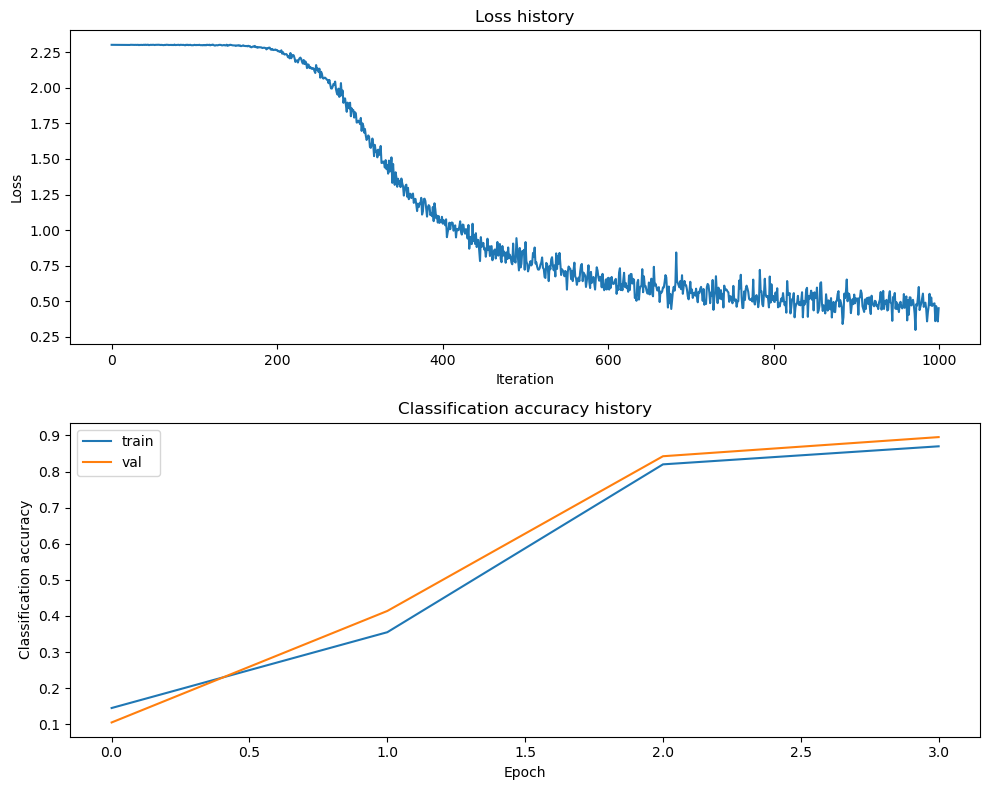
\includegraphics[width=\linewidth]{img/output3.png}
\caption{학습 과정에서의 훈련 손실과 분류 정확도}
\end{figure}

훈련 손실은 최적화 과정 동안 꾸준히 감소하며, 훈련 정확도와 검증 정확도 모두 에폭이 진행됨에 따라 증가한다. 훈련 정확도와 검증 정확도 사이의 차이가 크지 않다는 점은 모델이 심각한 과적합 없이 비교적 잘 학습되었음을 보여준다. 이러한 결과는 제안된 2층 신경망(two-layer neural network)이 손글씨 숫자 분류를 위해 의미 있는 정보를 효과적으로 학습할 수 있음을 보여준다.

\section{Discussion}

이 결과는 비교적 단순한 2층 신경망이라 하더라도 손글씨 숫자 분류에서 충분히 좋은 성능을 낼 수 있음을 보여준다. 은닉층의 크기를 증가시키면 모델의 표현 능력이 향상되었으며, 학습률과 정규화 값을 적절히 조정함으로써 학습을 안정화하고 성능을 개선할 수 있었다. 그러나 성능은 이전에 연습했던 더 깊은 CNN 모델보다 여전히 낮은 것으로 보인다. CNN은 일반적으로 이미지 인식 작업에서 널리 사용된다. 향후에는 더 깊은 네트워크 구조, 합성곱 층(convolution layers), 혹은 dropout과 같은 추가적인 정규화 기법을 도입하여 성능을 개선할 수 있을 것이다.

\end{document}
